\documentclass[a4paper]{article}

\usepackage{INTERSPEECH2016}

\usepackage{graphicx}
\graphicspath{ {images/} }
\usepackage{amssymb,amsmath,bm,bbm}
\usepackage{hyperref}
\usepackage{textcomp}
\usepackage{algorithm}
\usepackage{algpseudocode}

\def\vec#1{\ensuremath{\bm{{#1}}}}
\def\mat#1{\vec{#1}}
\DeclareMathOperator{\unif}{Unif}


\sloppy % better line breaks
\ninept

\title{Progress Update: Query Selection based on Latent Space Sampling}

%%%%%%%%%%%%%%%%%%%%%%%%%%%%%%%%%%%%%%%%%%%%%%%%%%%%%%%%%%%%%%%%%%%%%%%%%%
%% If multiple authors, uncomment and edit the lines shown below.       %%
%% Note that each line must be emphasized {\em } by itself.             %%
%% (by Stephen Martucci, author of spconf.sty).                         %%
%%%%%%%%%%%%%%%%%%%%%%%%%%%%%%%%%%%%%%%%%%%%%%%%%%%%%%%%%%%%%%%%%%%%%%%%%%
%\makeatletter
%\def\name#1{\gdef\@name{#1\\}}
%\makeatother
%\name{{\em Firstname1 Lastname1, Firstname2 Lastname2, Firstname3 Lastname3,}\\
%      {\em Firstname4 Lastname4, Firstname5 Lastname5, Firstname6 Lastname6,
%      Firstname7 Lastname7}}
%%%%%%%%%%%%%%% End of required multiple authors changes %%%%%%%%%%%%%%%%%

\makeatletter
\def\name#1{\gdef\@name{#1\\}}
\makeatother \name{{\em Benjamin Killeen}}

\address{University of Chicago \\
  {\small \tt killeen@uchicago.edu}
}

\begin{document}
\maketitle

\begin{abstract}
  The advent of deep learning has facilitated remarkable success on increasingly
  complex tasks. Large datasets are integral to this success, providing example
  labels which guide training, but these labels are not always readily
  available. The field of active learning addresses this issue by considering
  ``curious'' learners which iteratively select query sets that, when annotated,
  will most inform training. Crucially, this selection depends upon the
  performance of a supervised learner on already-labeled examples, initially
  selected randomly. Using techniques from unsupervised learning, our approach
  leverages the unlabeled data to inform both query selection as well as
  supervised training. Using an auto-encoder (AE), we consider various sampling
  strategies in the learned latent space which will produce informative
  examples. We further investigate the transfer of knowledge from the AE to a
  supervised learner, in this case a classifier.
\end{abstract}
\noindent{\bf Index Terms}: active learning, unsupervised learning, computer
vision

\section{Introduction}
\label{sec:introduction}

The collection and annotation of large datasets has been critical to the success
of deep learning. Wherever such a dataset is available, it seems, the focus of
the community eventually results in a supervised learner with high performance
\emph{on that dataset}. Although that performance may extend to examples from
similar tasks, many application domains are outside the scope of established
datasets, and relevant annotations may not exist at all. This is the case
especially for scientific image analysis, where the unique nature of each
experiment sets it apart from conventional tasks and the labeling itself is the
ultimate goal. In this context, one aims to train a supervised learner on as few
labeled examples as possible, possibly leveraging the unlabeled data to do so.

% \section{Related Work}
% \label{sec:related-work}

\section{Method}
\label{sec:method}

\begin{figure*}
  \centering
  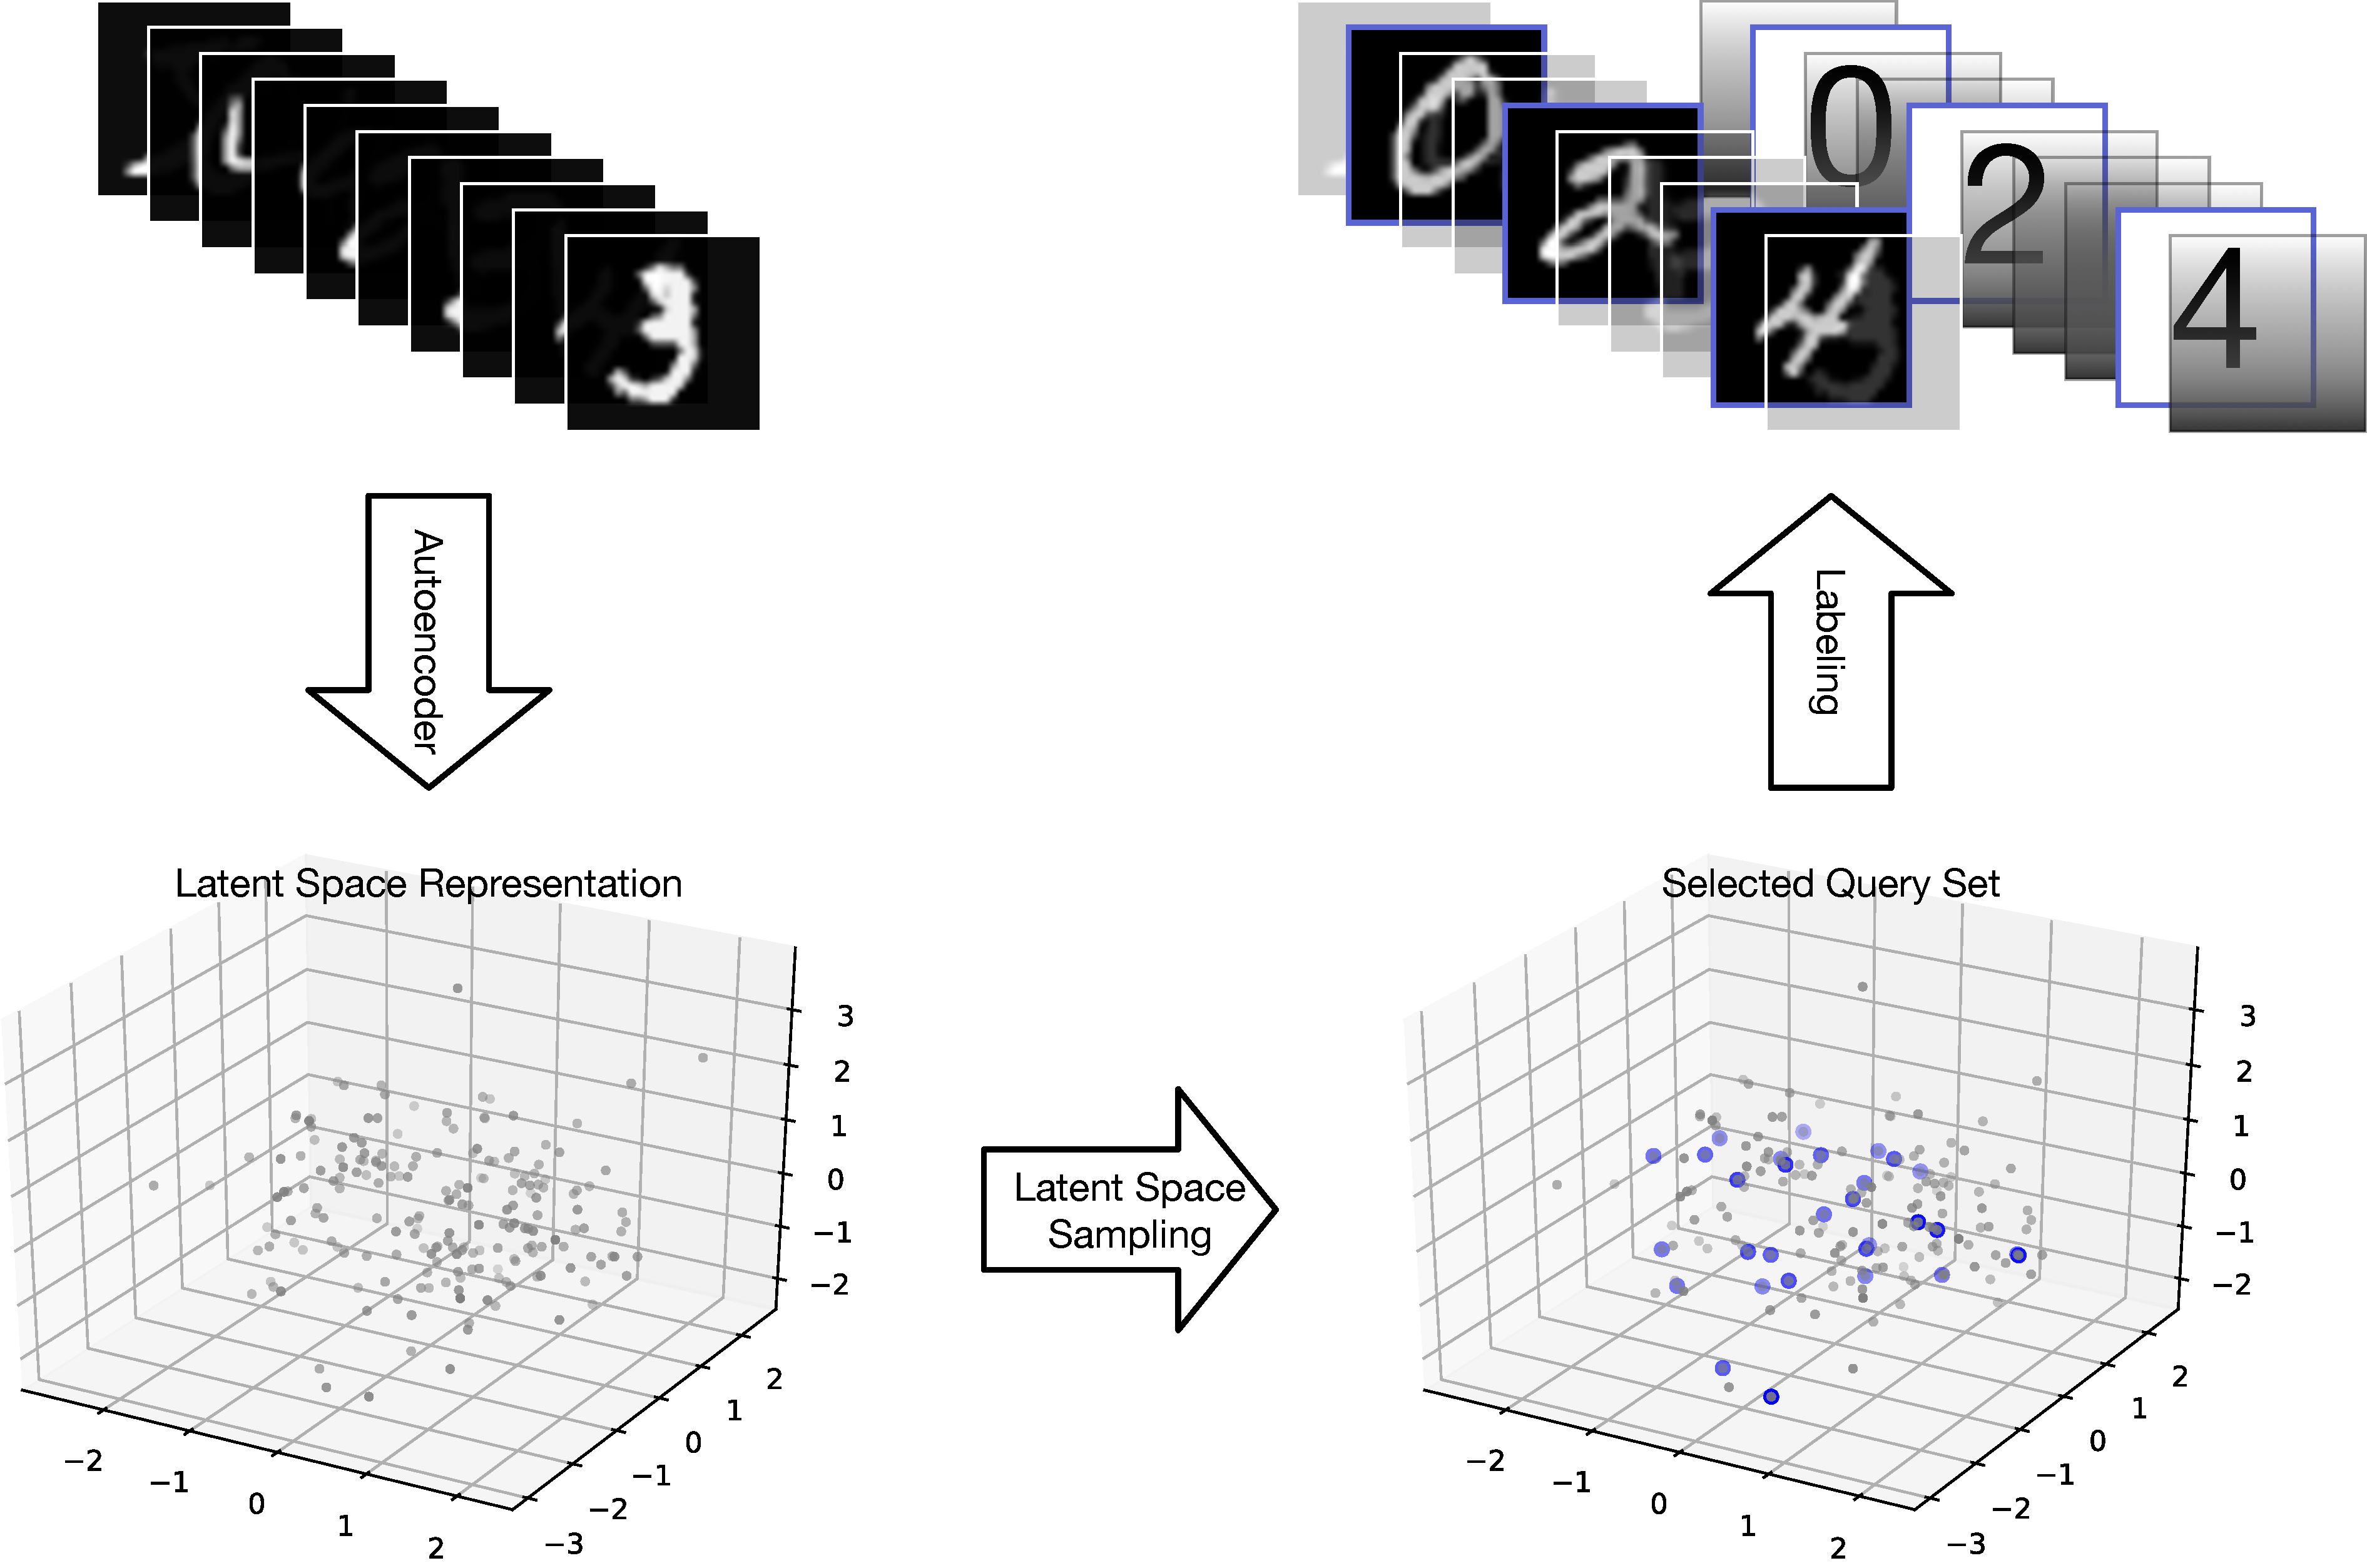
\includegraphics[width=0.9\linewidth]{overview}
  \caption{an overview of the query selection process. Given a large, unlabeled
    dataset, we train an autoencoder to generate latent space representations of
    each example. Next, the ``latent space sampling'' identifies examples which
    are well-spread-out in the low-dimensional encoding. Finally, the selected
    examples in the original dataset are labeled for training.}
  \label{fig:overview}
\end{figure*}

Given the nature of this report, we separate the discussion of our envisioned
method, in Section~\ref{sec:discussion}, with the description of our current
method, given here. This method is sub.ject to change, especially with regard to
the auto-encoder architecture and sampling strategy.

Latent space sampling uses a large unlabeled dataset to identify examples which
should be labeled, according to one of several strategies (which we expound on
in this report). Initially, we consider data matrix
$X \in \mathbb{R}^{N\times D}$, where $N$ is the number of examples and $D$ is
the dimensionality of each example. In our experiments, we use
$28 \times 28 \times 1$ images, so $D = 784$. From this unlabeled set, we use an
auto-encoder to learn a low-dimensional or latent space representation
$Z \in \mathbb{R}^{N\times L}$ of $X$, where $L$ is the dimensionality of the
latent space.

Currently, we use a convolutional auto-encoder (CAE) to learn a 10-dimensional
encoding of the dataset \cite{krizhevsky_imagenet_2012,
  goodfellow_deep_nodate}. The CAE consists of an encoder and a decoder. The
encoder uses multiple $3\times 3$ convolutional layers broken up with two
$2\times 2$ max-pooling to reduce the image dimensions to $7\times 7 \times 64$
in the last convolutional layer. This is followed by two dense layers with 1024
and $L$ nodes respectively. The decoder reverses this architecture, replacing
max-pool layers with $2\times 2$ transpose convolutions. In each layer, we use
the ReLU activation function, except for the encoder's final layer, the
``representation layer.'' The choice of activation for the representation layer
is driven by a combination of performance considerations---what generates good
encodings---as well as sampling considerations. Initially, we envisioned that
constraining the latent space to the hypercube $[0,1]^L$ would result in an
easily sampled representation with good spread.\footnote{This vision has since
  changed. See Section~\ref{sec:discussion} for details.} Experiments with the
sigmoid activation function proved unsatisfying, and so following Nair and
Hinton's Rectified Linear Unit \cite{nair_rectified_nodate}, we employ a clipped
linear unit (CLU) given by $f(x) = \min(1, \max(0,x))$, in our initial
experiments. This choice was made in order to guarantee a hypercube constrained
representation $Z \in [0,1]^{N\times L}$ while still providing the performance
advantages of the ReLU.

Once we obtain $Z$, we select a sampling or index set $Q \subseteq [N]$ based on
the distribution of $Z$. One strategy, which we employ in our preliminary
experiments, is to sample from this space according to a random uniform
distribution. As described in Algorithm~\ref{alg:uniform-sampling}, we draw a
point $z \in [0,1]^L$ uniformly and, if any data-point representation $z_i$
exists within a given distance $d(z,z_i)$, then we add $i$ to the query
set. Figure~\ref{fig:overview} provides an overview of this representation
learning and sampling process.

\begin{algorithm}
  \begin{algorithmic}[1]
    \Require encoding $Z \in [0,1]^{N \times L}$, distance metric
    $d : [0,1]^{2 \times L} \rightarrow \mathbb{R}$, distance threshold
    $t \in \mathbb{R}$, $n \in \mathbb{N}$.
    \State $Q \gets \{\}$
    \While {$|Q| < n$}
    \State Draw $z \in [0,1]^L \sim \unif^L(0,1)$
    \For {$z_i \in Z$}
    \Comment the $i$th row of $Z$
    \If {$d(z, z_i) < t$}
    \State $Q \gets Q \cup \{i\}$
    \EndIf
    \EndFor
    \EndWhile
    \State \Return $Q$
  \end{algorithmic}
  \caption{Approximate a uniform sampling of the latent-space hypercube
    $[0,1]^L$ from the encoding $Z$.}
  \label{alg:uniform-sampling}
\end{algorithm}

\section{Results}
\label{sec:results}

Although our main work until now has focused on implementation, we have some
early results of training that are worth showing. Firstly, we visualize the
behavior of an auto-encoder trained with $L = 10$. This auto-encoder was trained
for 20 epochs on the 50,000 image training set. It achieved a mean absolute
error on the test set of 0.0604. Figure~\ref{fig:autoencoder-visualization}
shows decodings of points in latent-space, varying a different dimension in each
row of the image. As can be seen, the representation produces many images that
are meaningful, but it does not fully explore the available space as might be
desired for our purposes.
z
\begin{figure}
  \centering
  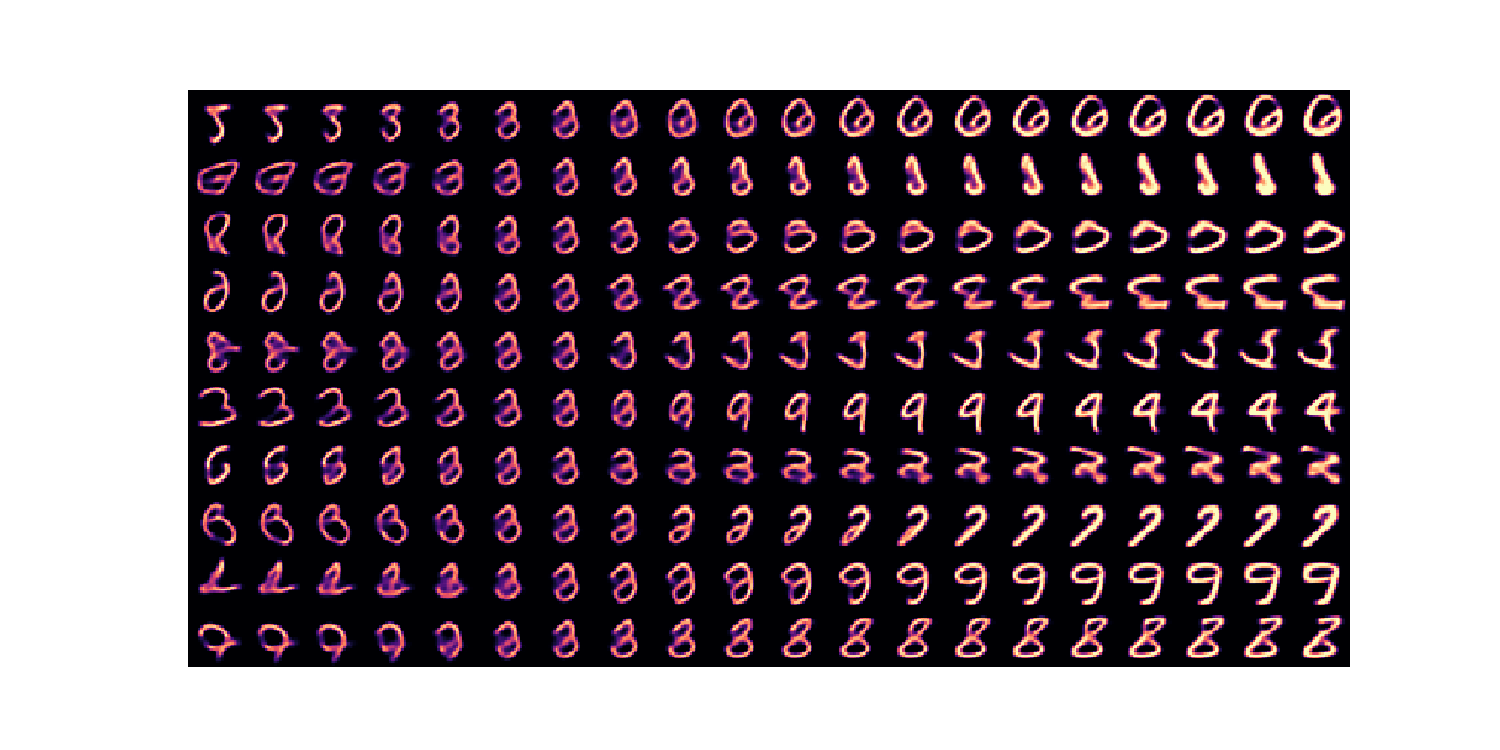
\includegraphics[width=\linewidth]{visualize_decoding}
  \caption{a visualization of the latent space $[0,1]^{10}$ learned by a simple
    convolutional autoencoder. The $i$th row corresponds to variation of the
    $i$th latent dimension from $0$ to $1$, fixing all other coordinates at
    $0.3$.}
  \label{fig:autoencoder-visualization}
\end{figure}

Sampling the latent representation $Z$ for 1000 examples according to our
method, we trained a simple convolutional classifier from scratch. This achieved
93.1\% accuracy on the 10,000 example test set. Although seemingly promising, we
note that a random sampling of the training set produced similar
results. Additionally, this preliminary finding trained the classifier from
scratch, without using any transfer learning.

\section{Discussion}
\label{sec:discussion}

Because of the difficulties we face with a simple CAE, we plan to implement a
variational auto-encoder (VAE) with convolution layers, restricting the
latent-space to an even lower dimension such as $L=2$ in the hopes of producing
a more meaningful and easily-sampled $Z$, while still using
Algorithm~\ref{alg:uniform-sampling}. After this step, it should no longer be
necessary to restrict the representation layer to the hypercube $[0,1]^L$.

Furthermore, we have some interest in exploring latent-space points which are
not in the original training set. If time allows, we plan to use the decodings
of regularly sampled points in the latent space as a training set for a
classifier, either employing an actual human annotator to provide labels for
these novel examples or using a separate classifier trained on the full dataset
to simulate a human labeler.

% \section{Conclusions}
% \label{sec:conclusion}

% \section{Acknowledgements}
% \label{sec:acknowledgements}


\newpage
\eightpt
\bibliographystyle{IEEEtran}

\bibliography{report}

\end{document}

%%% Local Variables:
%%% mode: latex
%%% TeX-master: t
%%% End:
